\documentclass[12pt]{Qual}
\usepackage{preamble}

\name{Kayla Orlinsky}
\course{Real Analysis Exam}
\term{Fall 2018}
\hwnum{Fall 2018}

\begin{document}

\begin{problem} $\,$
Let $f:[0,1]\to\mathbb{R}$ be an absolutely continuous function. Let $$g(x)=\int_0^1f(xt)dt,\qquad x\in[0,1].$$ Show that $g$ is an absolutely continuous function.
\end{problem}


\begin{solution}$\,$
Let $M\in\mathbb{R}$ and $$F_M=\{x\in[0,1]\,:\,|f(x)|\ge M\}.$$ Now, on $F_M^c$, $|f(x)|<M$. However, since $f(x)>0$ a.e., we have that for all $\varepsilon>0$, there exists $\delta>0$, so $$S=\{x\in [0,1]\,:\,|f(x)|>\delta\}$$ has measure $m(S)>1-\frac{\varepsilon}{2}$. So $m(S^c\cap[0,1])<\frac{\varepsilon}{2}$

Then $$\int_{E_k}f(x)dx\ge\int_{E_k\cap F_M^c\cap S}f(x)dx\ge\int_{E_k\cap F_M^c\cap S}\delta dx=\delta m(E_k\cap F_M^c S).$$

Therefore, since the left tends $0,$ we get that $$\lim_{k\to\infty}m(E_k\cap F_M^c\cap S)\to0.$$

Now, take $K$ so that for all $k\ge K$, $m(E_k\cap F_M^c\cap S)<\frac{\varepsilon}{2}$, then \begin{align*}
    m(E_k\cap F_M^c)&=m(E_k\cap F_M^c\cap S)+m(E_k\cap F_M^c\cap S^c)\\
    &<m(E_k\cap F_M^c\cap S)+\frac{\varepsilon}{2}\\
    &<\frac{\varepsilon}{2}+\frac{\varepsilon}{2}\\
    &=\varepsilon
\end{align*}

Thus, $m(E_k\cap F_M^c)\to0$ as $k\to\infty.$

Finally,
\begin{align*}
    \int_{E_k}f(x)dx&=\int_{E_k\cap F_M}f(x)dx+\int_{E_k\cap F_M^c}f(x)dx\\
    &\ge\int_{E_k\cap F_M}f(x)dx+\int_{E_k\cap F_M^c}f(x)dx\\
    &\ge\left|\int_{E_k\cap F_M}Mdx\right|+\int_{E_k\cap F_M^c}f(x)dx\\
    &=Mm(E_k\cap F_M)+\int_{E_k\cap F_M^c}f(x)dx
\end{align*}

and since $\displaystyle \int_{E_k}f(x)dx\to0$ and $m(E_k\cap F_M^c)\to0$ as $k\to\infty$, and since $f(x)<\infty$ on $E_k\cap F_M^c$, $\displaystyle \int_{E_k\cap F_M^c}f(x)dx\to0$ as $k\to\infty$ and so at last, $m(E_k\cap F_M)\to0$ as $k\to\infty.$
\end{solution}
\newpage




\begin{problem} $\,$
Let $f\in L^1(\mathbb{R})$, and let $$S_n(x)=\frac{1}{n}\sum_{j=0}^{n-1}f\left(x+\frac{j}{n}\right),\qquad x\in\mathbb{R},$$ $$S(x)=\int_x^{x+1}f(y)dy,\qquad x\in\mathbb{R}.$$ Show that $f_n\to f$ in $L^1(\mathbb{R}).$

\begin{mybox}
***We assume that the question meant to say ``Show that $S_n\to S$ in $L^1(\mathbb{R})$'' since no $f_n$ is ever defined.
\end{mybox}
\end{problem}


\begin{solution}$\,$
First, we note that $$\lim_{n\to\infty}S_n(x)=S(x)$$ as a Riemann integral. Now, since $f$ is Lebesgue integrable, it is bounded almost everywhere and since it is Lebesgue measurable, it is continuous almost everywhere.

Namely, we have that $S(x)$ the Riemann integral, will equal the Lebesgue integral for a.e. $x.$

We will apply DCC to $|S_n(x)-S(x)|$
\begin{enumerate}
    \item $|S_n(x)-S(x)|$ is measurable.
    \item $$\lim_{n\to\infty}|S_n(x)-S(x)|=|\lim_{n\to\infty}S_n(x)-S(x)|=0$$ by definition of the Riemann integral. And as stated before, the Riemann integral and Lebesgue integral agree a.e.
    \item $|S_n(x)-S(x)|\le 2|S(x)|\in L^1$ for all $n$ and $S\in L^1$ since $f\in L^1$ so by Tonelli \begin{align*}
        \int_\mathbb{R}|S(x)|dx&\le \int_\mathbb{R}\int_x^{x+1}|f(y)|dydx\\
        &=\int_\mathbb{R}\int_0^1|f(u-x)|dudx\qquad u=y-x\\
        &=\int_0^1\int_\mathbb{R}|f(u-x)|dxdu\qquad\text{ Tonelli}\\
        &=\int_0^1Mdu\\
        &=M<\infty
    \end{align*}
    Where $M=\int|f(x)|dx<\infty$ since $f\in L^1.$
\end{enumerate}

Therefore, by DCC, $$\lim_{n\to\infty}\int|S_n(x)-S(x)|dx=\int\lim_{n\to\infty}|S_n(x)-S(x)|dx=0$$

So $S_n\to S$ in $L^1.$
\end{solution}
\newpage



\begin{problem} $\,$
Assume that $f_n$ is a sequence of integrable functions on $\mathbb{R}$ such that $$\lim_{n\to\infty}\int f_n(x)g(x)dx=g(0)$$ for all $g$ continuous with compact support.

Prove that $f_n$ is not a Cauchy sequence in $L^1(\mathbb{R}).$
\end{problem}


\begin{solution}$\,$
Let $g(x)$ be a smoothed out characteristic function on $[-1,1]$ times some constant $a.$

\begin{center}
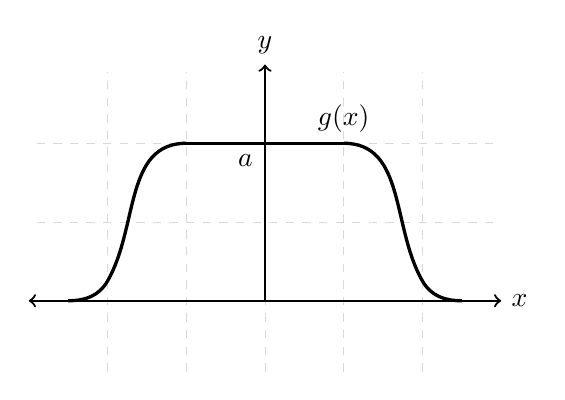
\begin{tikzpicture}
\draw[help lines, color=gray!30, dashed] (-2.9,-0.9) grid (2.9,2.9);
\draw[very thick] (-1,2) -- (1,2) node[above]{$g(x)$};
\draw[very thick] (-0.1,2) -- (0.1,2) node[below,xshift=-0.35cm,yshift=0cm]{$a$};
\draw[very thick] (-2.5,0) to[out=0, in=-120] (-2,0.25) to[out=60, in=180](-1,2);
\begin{scope}[xscale=-1,xshift=0cm]
\draw[very thick] (-2.5,0) to[out=0, in=-120] (-2,0.25) to[out=60, in=180](-1,2);
\end{scope}
\draw[<->, thick] (-3,0)--(3,0) node[right]{$x$};
\draw[->, thick] (0,0)--(0,3) node[above]{$y$};
\end{tikzpicture}
\end{center}

Now, because $\int f_ngdx\to g(0)$ regardless of what $g$ is doing away from $0$, we claim that the $\int f_ndx$ is $1$ near $0$ and $0$ everywhere else.

First, let $\varepsilon>0$ and let $a=1$. Then $$\lim_{n\to\infty}\int_{[-\varepsilon,\varepsilon]}f_n(x)dx=\lim_{n\to\infty}\int_{[-\varepsilon,\varepsilon]}f_n(x)g(x)dx=g(0)=1.$$

Now, shift and stretch $g$ so that $g(0)=0$ and $g(x)=1$ is nonzero on some $[-M,-\varepsilon]$ large negative interval.

Then $$\lim_{n\to\infty}\int_{[-M,-\varepsilon]}f_n(x)dx=\lim_{n\to\infty}\int_{[-M,-\varepsilon]}f_n(x)g(x)dx=g(0)=0.$$

Similarly, we get that $\displaystyle_{[\varepsilon,M]}f_n(x)dx\to 0$. Namely, for large $n$, the integrals have value only near $0.$

Thus, for all $\varepsilon>0$, there exists $N>0$ such that $$\left|\int f_n(x)dx-1\right|<\varepsilon$$ for all $n\ge N.$

However, for all $\delta<0$, we have that $$\left|\int_{[-\delta,\delta]} f_n(x)dx-1\right|<\varepsilon$$ for all $n\ge N.$

Now, $L^1$ is complete, so if $f_n\not\to f$ for any measurable function $f$ in $L^1$, then $f_n$ cannot be cauchy in $L^1.$

Let $f$ be any measurable function, and $f_n\to f$ in $L^1$, then taking $n$ large enough we get that  \begin{align*}
    \varepsilon>\int_{[-\delta,\delta]}|f_n(x)-f(x)|dx&\ge\left|\int_{[-\delta,\delta]}f_n(x)-f(x)dx\right|\\
    &\ge\left|\int_{[-\delta,\delta]}f_n(x)dx\right|-\int_{[-\delta,\delta]}|f(x)|dx\\
    &>1-\varepsilon-\int_{[-\delta,\delta]}|f(x)|dx
\end{align*}

Namely, $$\int_{[-\delta,\delta]}|f(x)|dx=1\qquad\text{ for all }\delta$$

However, since $f_n\in L^1$, it must be that $f\in L^1$ and this is clearly a contradiction since taking $\delta\to0$ we cannot have that $\{x\,|\,|f(x)|=\infty\}$ is null.

Thus, $f_n$ does not converge to any $L^1$ function in $L^1$, so it cannot be a Cauchy sequence in $L^1.$
\end{solution}
\vspace{0.5cm}

\end{document}
